%%%%%%%%%%%%%%%%%%%%%%%%%%%%%%%%%%%%%%%%%%%%%%%%%%%%%%%%%%%%%%%%%%%
%%%%%%%%%%%%%%%%%%%%%%%%%%%%  DEPLOYER  %%%%%%%%%%%%%%%%%%%%%%%%%%%%%%%%
%%%%%%%%%%%%%%%%%%%%%%%%%%%%%%%%%%%%%%%%%%%%%%%%%%%%%%%%%%%%%%%%%%%
Characteristics of GPOD and ISIPOD. First, the main ones that both have in common are shown, secondly, the few differences between them are listed:
\begin{itemize}
\item Main features
\begin{itemize}
\item Provide deployment status signal.
\item No battery needed nor external power source
\item No pyrotechnics
\item Protect the CubeSat from external environmental impact
\item Mechanically interfaces with the CubeSats by means of guidelines
\item Mechanically interfaces with the launch vehicle by means of standard fasteners
\item Qualified for multiples launch vehicles
\end{itemize}
\item ISIPOD 
\begin{itemize}
\item The satellites are fully enclosed inside the deployer, so once the CubeSat is fit in, there is no access to it (see image \ref{fig:gull})
\item Electrically interfaces with launch vehicle for telemetry
\end{itemize}
\item GPOD
\begin{itemize}
\item Accessible panels: all the side panels allow the access to the integrated CubeSat (see image \ref{fig:tiger}). This means that the entire area between the guide rails over the entire CubeSat length may be freely accessed. 
\item The price for a single deployer 3U is 16000 euros. 
\end{itemize}
\end{itemize}

\begin{figure}[h!]
\centering 
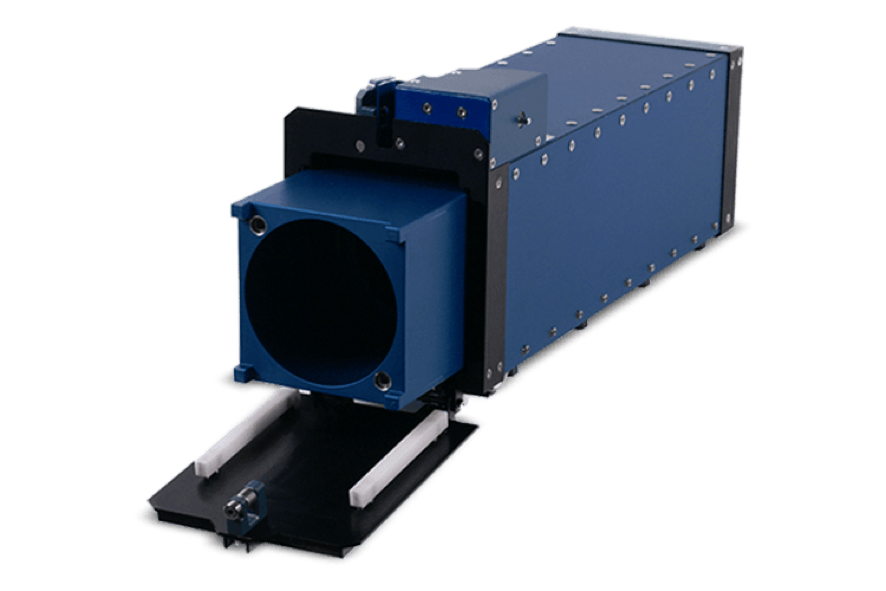
\includegraphics[scale=0.7]{./sections/Constellation_Deployment/S3-Deployer/Images_S3/Picture_1_S3.png} 
\caption{ISIPOD}
\label{fig:gull}
\end{figure}

\begin{figure}[h!]
\centering 
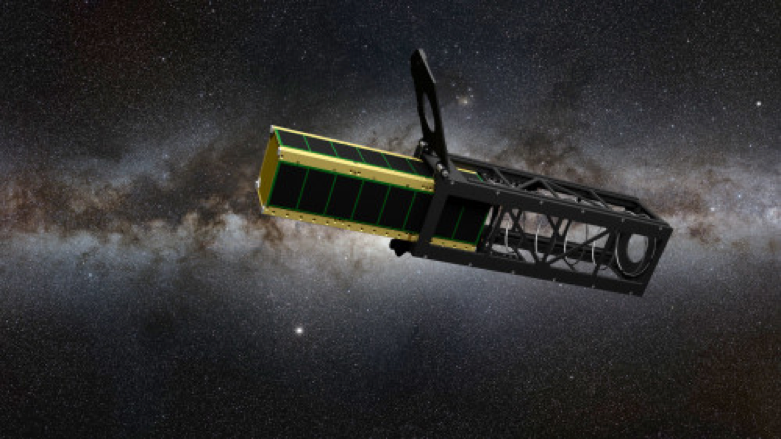
\includegraphics[scale=0.7]{./sections/Constellation_Deployment/S3-Deployer/Images_S3/Picture_2_S3.png} 
\caption{GPOD}
\label{fig:tiger}
\end{figure}
	
